% !TEX encoding = UTF-8
% !TEX TS-program = pdflatex
% !TEX root = ../tesi.tex

%**************************************************************
\chapter{Descrizione dello stage}
\label{cap:descrizione-stage}
%**************************************************************

\intro{In questa sezione verrà trattato come si è svolto lo stage presso EsignWorld, considerando gli obiettivi pianificati, discutendo dei possibili rischi e la comunicazione con il tutor aziendale.}\\

\section{Introduzione}
Lo stage presso EsignWorld aveva come scopo la creazione di un engine che monitorasse i ticket aperti dai clienti dell'azienda per capire se si fosse in procinto di violare le Service Level Agreement stipulate con tale cliente. \\
Per far ciò, ci si è andati a interfacciare a Redmine, prodotto usato internamente dall'azienda per la gestione di progetti e l'apertura di ticket. Grazie ad esso quindi, ci si è potuti sollevare la parte di gestione del ticket e dei clienti, focalizzandosi solo sulla parte di analisi e notifica. \\
Una volta ottenuti i dati da Redmine, l'engine doveva appunto analizzare i dati, confrontarli con le S.L.A. fornitegli per ogni cliente, e in caso si fosse vicini al violarle, o la violazione fosse già avvenuta, procedere a segnalarlo al responsabile, tramite molteplici canali di notifica (quali per esempio Telegram e Email). \\
Infine, il progetto doveva predisporre anche un API per la pubblicazione dei dati: tale API aveva come scopo un monitoraggio statistico dei ticket, delle segnalazioni e delle violazioni, e quindi mirava a preparare i dati per esempio per graficarli o manipolarli.


%**************************************************************
\section{Obiettivi del progetto}
\begin{itemize}
	\item Principali:
	\begin{enumerate}
		\item Studio e valutazione di componenti esterni ai quali interfacciarsi successivamente.
		\item Test e recupero dati dai servizi esposti da Redmine.
		\item Analisi di vari sistemi di notifica, come Telegram e Email.
		\item Redazione di un documento di Analisi dei Requisiti.
		\item Redazione di un documento di Progettazione Tecnica.
		\item Sviluppo/Codifica del progetto seguendo le norme di codifica aziendali.
		\item Redazione documentazione del progetto:
		\begin{enumerate}
			\item Manuale di manutenzione.
			\item Manuale di installazione.
			\item Documentazione API.
		\end{enumerate}
	\end{enumerate}
	\item Secondari:
	\begin{enumerate}
		\item Integrazione dell'API con l'applicativo ENAnalytics
		\item Integrazione della base di dati con l'applicativo Grafana
		\item Sviluppo di test di unità e di integrità
	\end{enumerate}
\end{itemize}


%**************************************************************
\section{Analisi preventiva dei rischi}

Durante la fase di analisi iniziale sono stati individuati alcuni possibili rischi a cui si poteva andare incontro.
Si è quindi proceduto a elaborare delle possibili soluzioni per far fronte ad essi.\\


\begin{risk}{Tecnologie nuove}
    \riskdescription{le tecnologie consigliate per lo sviluppo del progetto erano nuove, causando un'inevitabile inesperienza nel loro utilizzo}
    \risksolution{è stato predefinito un periodo iniziale di formazione personale per le tecnologie che son state poi utilizzate per lo sviluppo, così da aver tempo di familiarizzarci leggermente e arrivare alla codifica con le nozioni base già apprese}
\end{risk}
\begin{risk}{Sistemi esterni}
	\riskdescription{il progetto richiede di interfacciarsi con sistemi esterni (quali per esempio Redmine) mai usati prima e che potrebbero avere una documentazione non esaustiva}
	\risksolution{è stata predefinito un periodo iniziale di formazione personale sui sistemi ai quali ci si è interfacciati durante la codifica, così da avere già una chiara visione del loro funzionamento e delle feature che mettono a disposizione}
\end{risk}
\begin{risk}{Gestione dello smart working}
	\riskdescription{lo stage si è tenuto interamente da remoto, portando quindi a un potenziale rischio di mancanza di comunicazione, che avrebbe potuto portare a un'incerta comprensione degli obbiettivi dello stage e del progetto affrontato}
	\risksolution{si è deciso di avere un meeting giornaliero con il tutor aziendale nelle prime fasi del progetto, così da esser sicuri che si arrivasse alle fasi finali (come la codifica) con tutti i chiarimenti necessari espletati}
\end{risk}
 


%**************************************************************

\subsection{Pianificazione}
	Di seguito sono elencate le varie fasi previste per lo stage e una loro stima oraria, in ordine cronologico:
	\begin{enumerate}
		\item \textbf{Conoscenze generali}: ($\sim$1 giorno) approfondimento e installazione degli ambienti di sviluppo e di versionamento, e abilitazione strumenti aziendali. 
		\item \textbf{Acquisizione degli standard aziendali}: ($\sim$1 giorno) esposizione dei servizi server Euronovate e dell'architettura della soluzione di firma Euronovate. 
		\item \textbf{Formazione personale}: ($\sim$5 giorni) formazione sul framework target per lo sviluppo, valutazione e test di componenti esterni (sistemi di notifica come email e messaggistica istantanea), istruzione sull'applicativo Redmine e recupero dati dai suoi servizi esposti.
		\item \textbf{Analisi dei requisiti}: ($\sim$4 giorni) analisi del tipo di informazioni da monitorare e successivamente da esporre/pubblicare, selezione dei sistemi e delle regole di notifica (e relativa frequenza di aggiornamento dati locali).
		\item \textbf{Progettazione tecnica}: ($\sim$5 giorni) stesura della specifica tecnica del Back-End, dei servizi esposti e degli oggetti di scambio.
		\item \textbf{Codifica}: ($\sim$18 giorni) sviluppo del prodotto seguendo le norme di codifica aziendali e potenzialmente test di unità e integrità.
		\item \textbf{Documentazione}: ($\sim$4 giorni) stesura manuale di manutenzione, manuale di installazione, e documentazione API.
		\item \textbf{Demo}: ($\sim$1 giorno) presentazione del prodotto sviluppato dall'azienda. 
	\end{enumerate}
	Il tutto può essere visualizzato nel seguente Gantt Chart:
	\begin{center}
		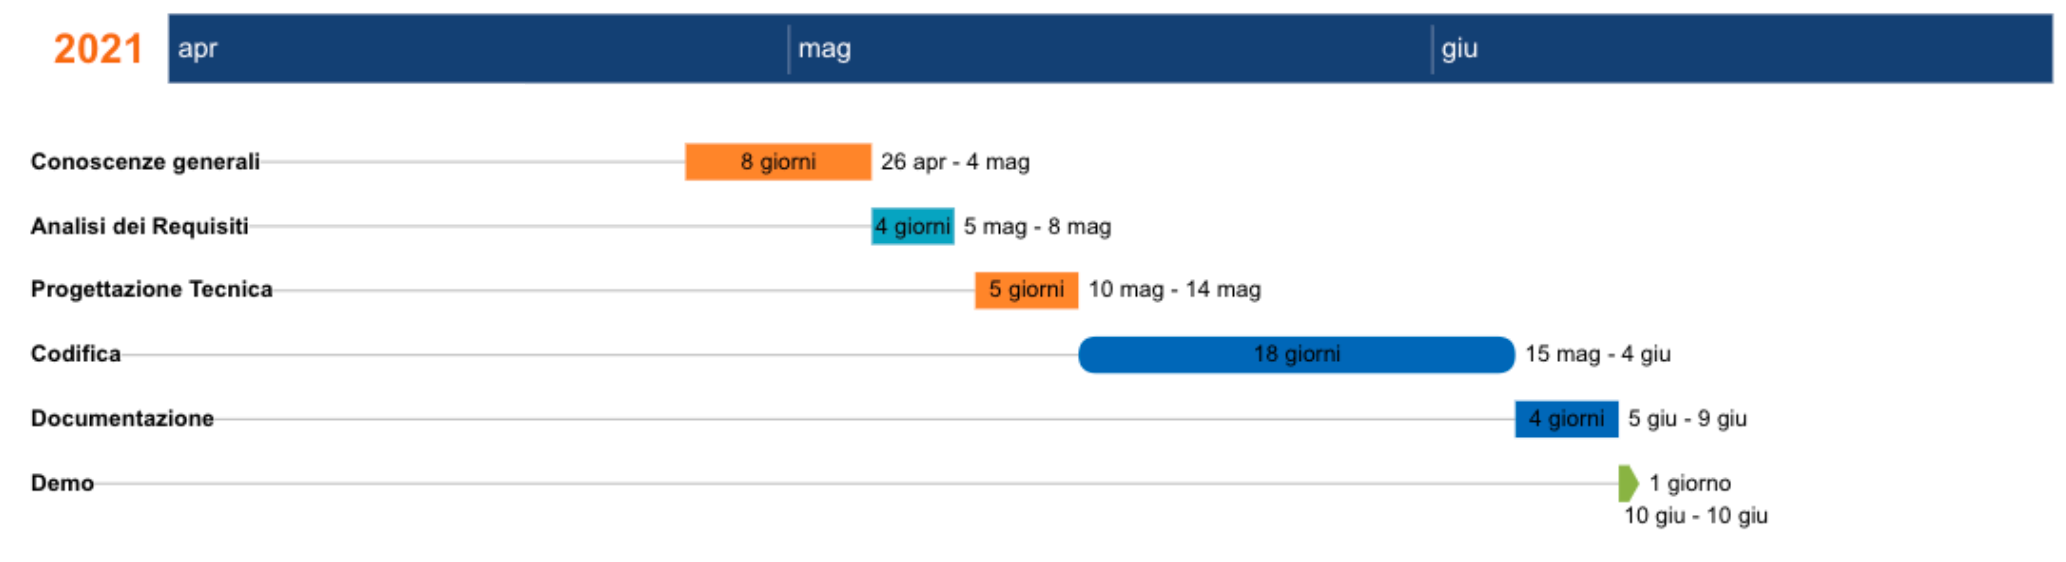
\includegraphics[keepaspectratio = true, width=15cm]{immagini/pianificazione.png}
		\captionof{figure}{Pianificazione dello stage}
	\end{center}
\iffalse
	\subsection{Suddivisione del carico di lavoro}
		\begin{center}
			\begin{table}[h!]
				\centering
				\begin{tabular}{c | c | c | c} 
					\textbf{Fase} & \textbf{Data inizio} & \textbf{Data fine} & \textbf{Durata}\\
					\hline
					Conoscenze generali   & 26/04/2021 & 04/05/2021 & 64 \\
					Analisi dei requisiti       & 05/05/2021 & 08/05/2021 & 32 \\
					Progettazione tecnica & 10/05/2021 & 14/05/2021 & 40 \\
					Codifica                       & 15/05/2021 & 04/06/2021 & 144 \\
					Documentazione         & 05/06/2021 & 09/06/2021 & 32 \\
					Demo                           & 10/06/2021 & 10/06/2021 & 8 \\
					\hline\hline
					\multicolumn{3}{l}{\textbf{Totale}} & 320 \\
				\end{tabular}
				\vspace{0.3cm}
				\caption{Tabella della suddivisione delle ore per ogni fase del progetto di stage}
			\end{table}
		\end{center}
\fi
		